% File: cambiamenti.tex
% Created: 2014/01/13
% Author: Tesser Paolo
% Email: p.tesser921@gmail.com
% 
%
% Modification History
% Version	Modifier Date	Author			Change
% ====================================================================
% 0.0.1		2015/01/13		Tesser Paolo	inserita sezione capitolo
% ====================================================================
%

\section{Cambiamenti e Aggiunte}
In questa sezione verranno descritti i cambiamenti apportati alla precedente versione del programma per permettere all'algoritmo di risoluzione di essere parallelizzato. \\
In generale non vengono effettuate particolari rivisitazioni della precedente struttura, ma vengono introdotte nuove gerarchie ed estese alcune precedentemente create. \\
Il client rappresentato dalla classe \textbf{PuzzleSolver} andrà modificato solo nella scelta della politica di esecuzione dell'algoritmo, che da sequenziale passerà a parallela utilizzando la nuova classe descritta nella sezione \ref{ssub:package_solver_1}.

	\subsection{Estensioni} % (fold)
	\label{sub:estensioni}
		\subsubsection{Package solver} % (fold)
		\label{ssub:package_solver_1}
		Questo package contiene le classi che gestiscono la risoluzione del puzzle. \\
		Viene estesa la gerarchia che comprendeva alla base l'interfaccia \textbf{SolverStrategy} e come sottotipo la classe \textbf{SolverAlgStrategy} con una nuova classe \textbf{SolverParStrategy} responsabile della risoluzione parallela del puzzle.
		La nuova classe avrà all'interno del metodo \textbf{executeSolve} il flusso di quali e quanti thread andranno lanciati per ordinare il puzzle.
		% subsubsection package_solver (end)
		
	% subsection estensioni (end)
	
	\subsection{Nuove gerarchie} % (fold)
	\label{sub:nuove_gerarchie}
		\subsubsection{Package solver} % (fold)
		\label{ssub:package_solver_2}
		Questo package contiene le classi che gestiscono la risoluzione del puzzle. \\
		In esso vengono aggiunte le classi che contengono l'attività logica che i diversi thread andranno ad eseguire. \\
		La gerarchia creata ha alla base una classe astratta \textbf{BasicThread}, che implementa l'interfaccia \textbf{Runnable}, utilizzata per memorizzare i membri condivisi da tutti i task come il riferimento all'oggetto condiviso dai Thread per comunicare tra loro o il riferimento all'oggetto Puzzle da risolvere. \\
		Viene estesa da \textbf{AngleTileThread}, \textbf{FirstColThread}, \textbf{RowThread}. \\
		\textbf{AngleTileThread} è il task che ha il compito di cercare e ordinare, nella struttura che contiene il puzzle risolto, il pezzo avente idWest e idNorth uguali a VUOTO e quello avente e idSouth uguali a VUOTO. \\
		\textbf{FirstColThread} è il task che ha il compito di ordinare la prima colonna del puzzle. Per farlo può partire dai precedenti pezzi trovati a seconda di quanto specificato nel paramentro attuale del task durante la sua creazione. I valori che potrà ricevere saranno: ``up'' per partire dal basso e salire fino alla metà della colonna, mentre ``down'' per partire dal basso e arrivare sempre fino alla metà. \\
		\textbf{RowThread} è il task che serve per riordinare tutte le righe del puzzle a partire dal primo elemento di ciascuna di essa. \\
		\\
		Tutti queste classi svolgono il loro compito nel metodo \textbf{run()}.
		% subsubsection package_solver (end)
		
		\subsubsection{Package logger} % (fold)
		\label{ssub:package_logger}
		Questo package contiene solamente una classe che mi serve per la gestione di un file testuale di log che viene usato per tracciare l'esecuzione del programma in alcuni punti. \\
		Essendo non importante ai fini delle richieste del proponente non ne verrà fornita una rappresentazione grafica.
		% subsubsection package_logger (end)
		
		\noindent
		\\ \\
		In seguito viene illustrato il package solver contenente sia la gerarchia ampliata degli algoritmi di risoluzione, sia quella dei Thread che vengono avviati per ordinare il puzzle.
		\begin{figure}[htbp]
			\centering
			\centerline{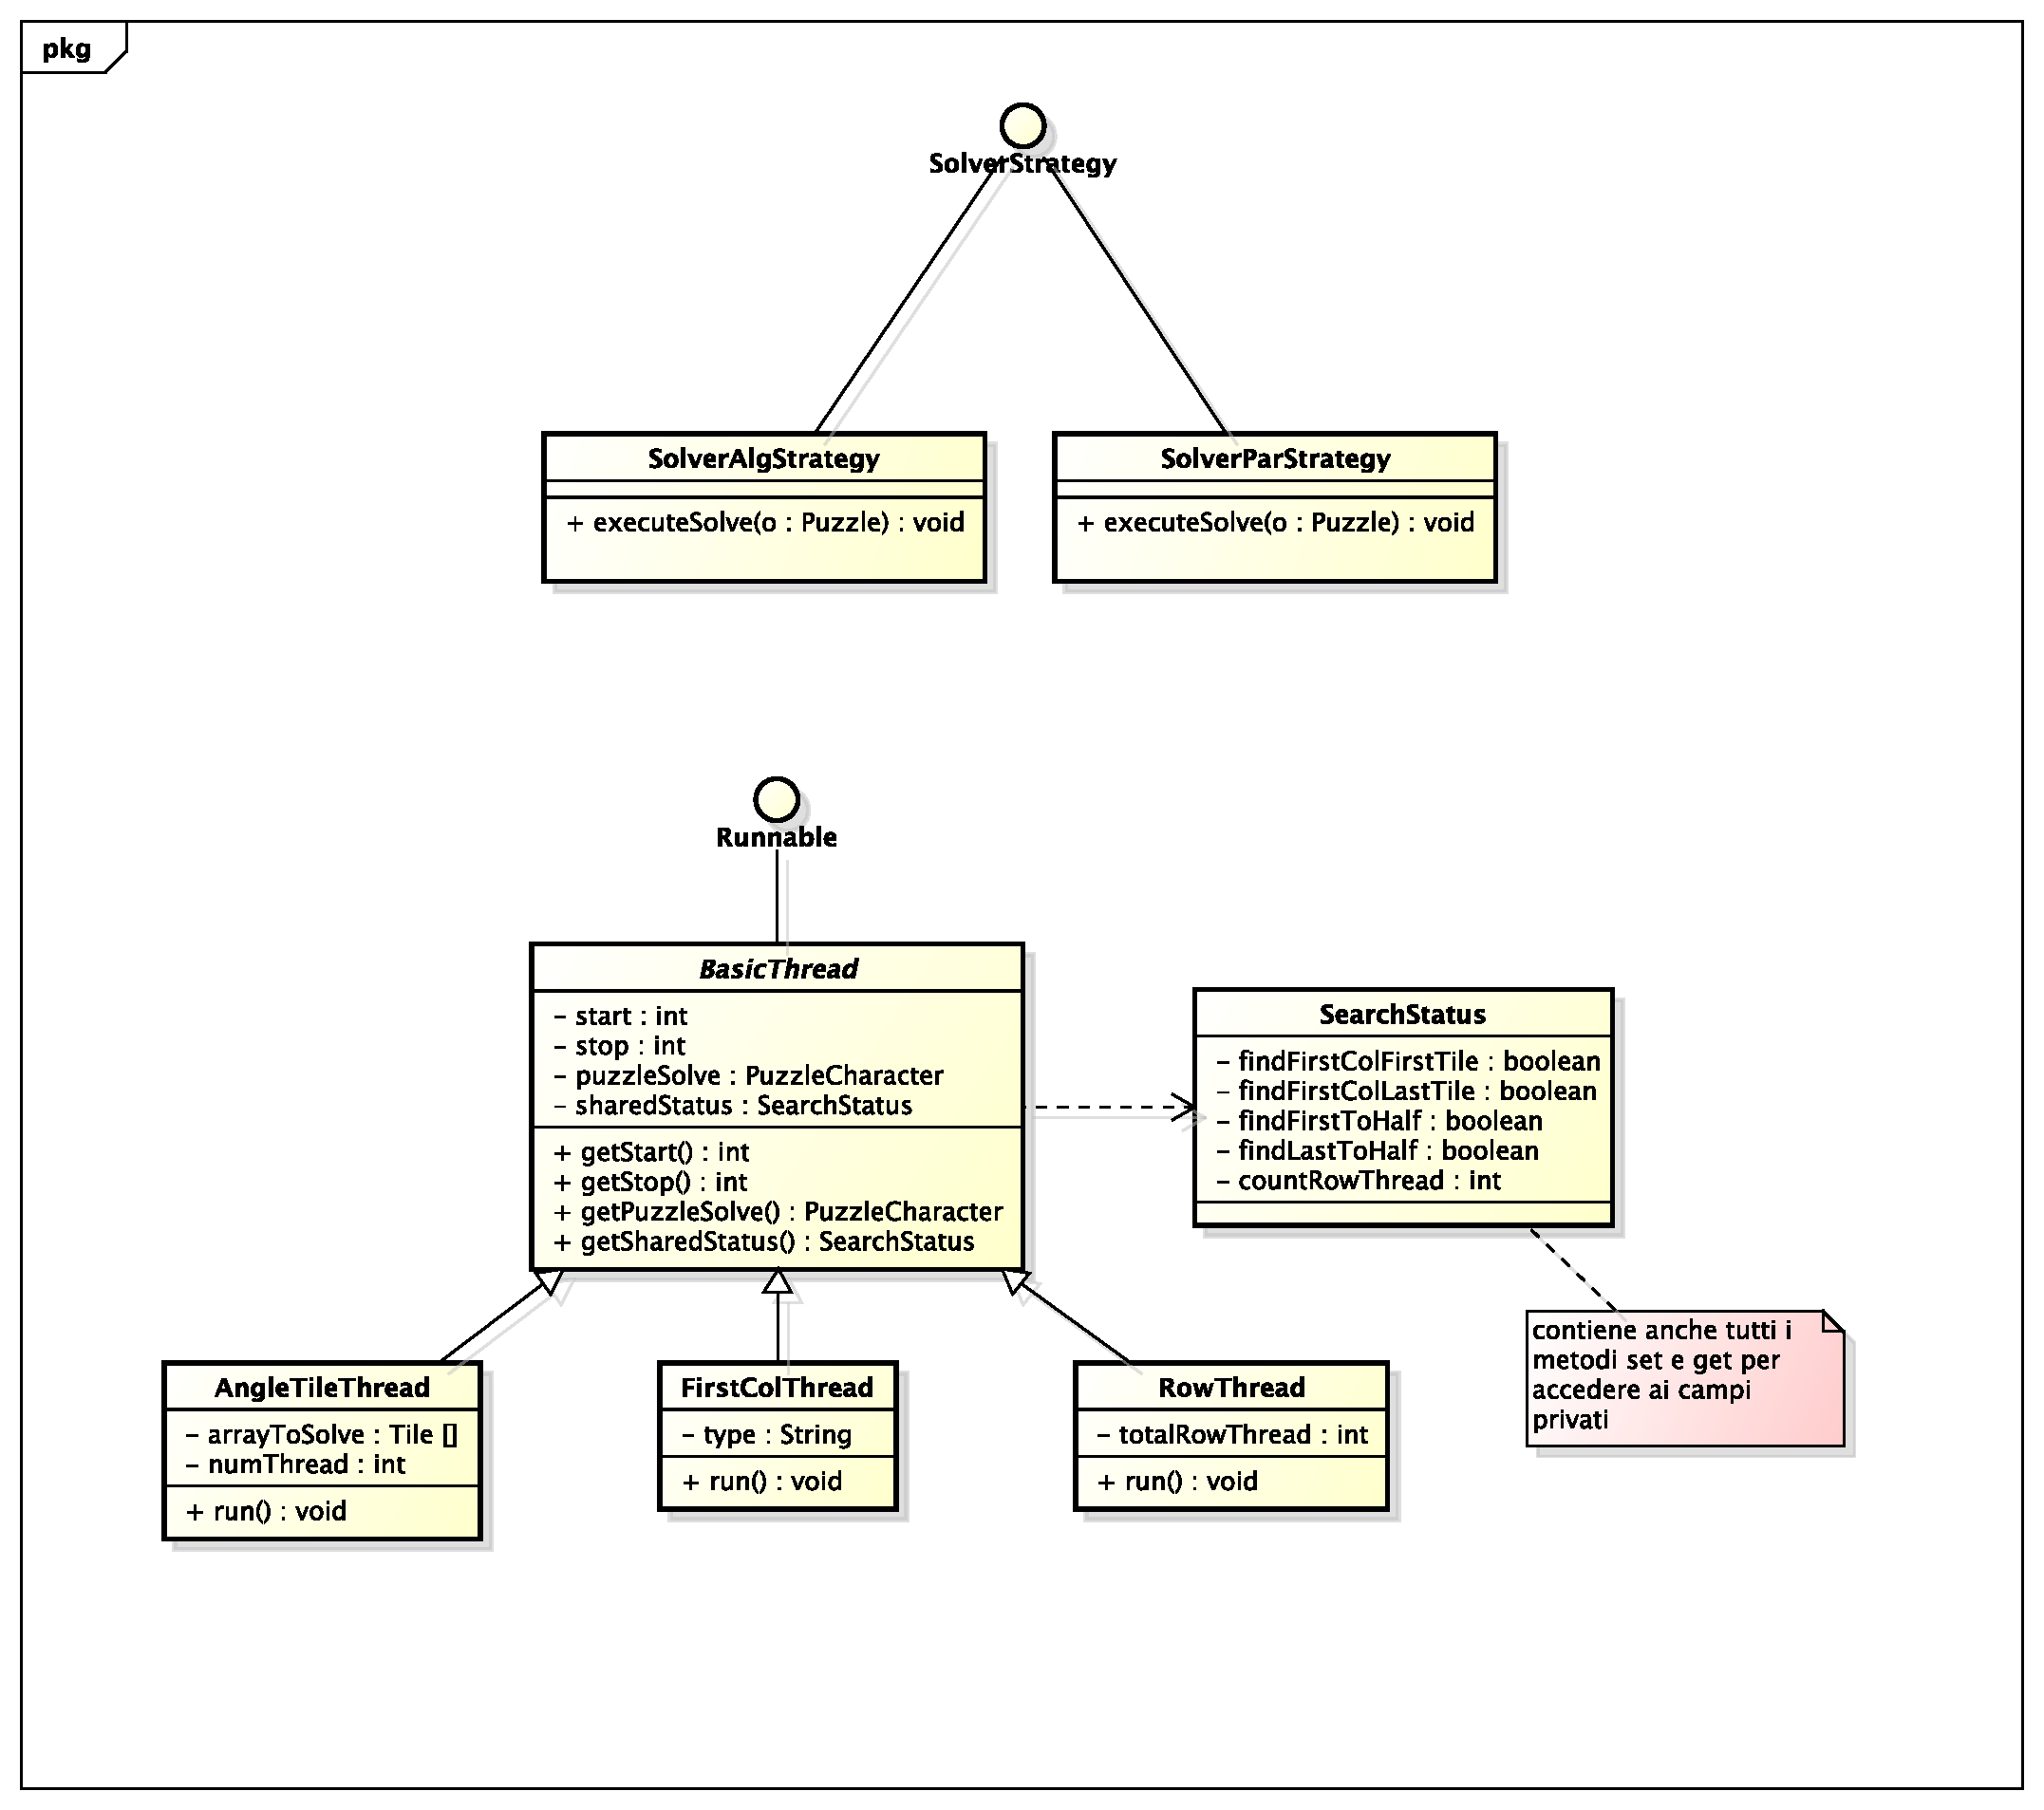
\includegraphics[scale=0.5]{img/solver.pdf}}
			\caption{Package Solver}
			\label{Package solver}
		\end{figure}
		
		
	% subsection nuove_gerarchie (end)

